\chapter{Related Works}

\section{PhoGPT}

\begin{table*}[!h]
    \centering
    \begin{tabular}{l|c|c}
    \hline 
    \textbf{Model} & \textbf{All truthful questions} & \textbf{Vietnam-specific} \\
    \hline
    PhoGPT-4B-Chat	& \underline{41.7	(83 / 199)}	& \textbf{43.5	(64 / 147)} \\
    %\hdashline
    GPT-4-0125-preview		& \textbf{44.7	(89 / 199)}		& 39.5	(58 / 147)  \\
    GPT-3.5-turbo		& 29.1	(58 / 199)		& 22.4	(33 / 147)  \\
    Gemini Pro 1.0		& 39.7	(79 / 199)		& 34.7	(51 / 147)  \\
    %\hdashline
    Vistral-7B-Chat		& 41.2	(82 / 199)		& \underline{42.9	(63 / 147)}  \\
    Sailor-7B-Chat		& 28.6	(57 / 199)		& 27.9	(41 / 147)  \\
    Sailor-4B-Chat		& 15.6	(31 / 199)		& 14.3	(21 / 147)  \\
    SeaLLM-7B-v2		& 20.6	(41 / 199)		& 13.6	(20 / 147)  \\
    VBD-Llama2-7B-50B-Chat		& 15.6	(31 / 199)		& 10.9	(16 / 147)  \\
    Vinallama-7B-Chat		& 11.1	(22 / 199)		& 8.2	(12 / 147)  \\
    Gemma-7B-it		& 8.0	(16 / 199)		& 6.1	(9 / 147)  \\
    \hline 
    \end{tabular}
    \caption{PhoGPT-4B-Chat and other models' performance on the truthful questions and Vietnam-specific questions tasks. The best model is listed in bold and second-best is listed in underlined.}
    \label{table:comparision}
\end{table*}

PhoGPT \cite{nguyen2024phogptgenerativepretrainingvietnamese} is a open-source state-of-the-art Transformer decoder-based model series for Vietnamese, including the base pre-trained monolingual model PhoGPT-4B and its chat variant, PhoGPT-4B-Chat. The base model, PhoGPT-4B, with exactly 3.7B parameters, is pre-trained from scratch on a Vietnamese corpus of 102B tokens, with an 8192 context length, employing a vocabulary of 20480 token types. The chat variant, PhoGPT-4B-Chat, is the modeling output obtained by fine-tuning PhoGPT-4B on a dataset of 70K instructional prompts and their responses, along with an additional 290K conversations. \par
The PhoGPT series has achieved state-of-the-art results on various Vietnamese NLP tasks in questions form as showed in \ref{table:comparision}


\section{Tiny Language Models}
The work of Yehui Tang et al. \cite{tang2024rethinkingoptimizationarchitecturetiny} introduces a series of experiments on Tiny Language Models based on Pangu, a large-scale  language model on Chinese and English. The authors propose a method to compress Pangu into Pangu-$\pi$-1B-pro and Pangu-$\pi$-1.5B-pro with 1B and 1.5B parameters, respectively. The experiments show that the small models can achieve competitive performance with a much smaller number of parameters compared to the original model as showed in Table \ref{tab:pangu_benchmark} and Figure \ref{fig:pangu_pi} \par

\begin{figure*}[!h]
    \centering
    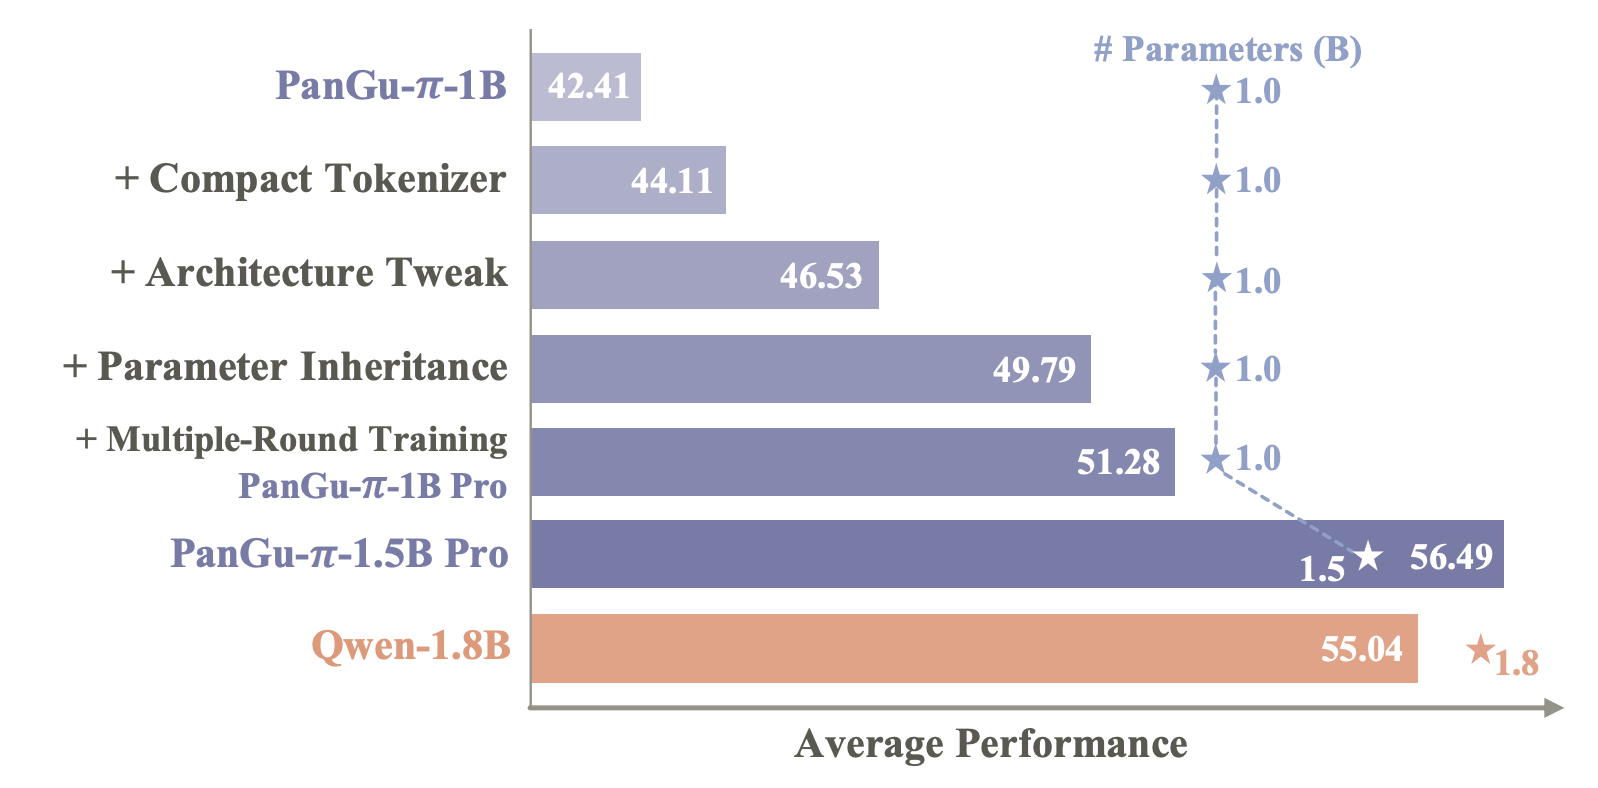
\includegraphics[width=0.8\textwidth]{Figures/pangu.png}
    \caption{Pangu-$\pi$-1B-pro and Pangu-$\pi$-1.5B-pro performance compared to other small model.}
    \label{fig:pangu_pi}
\end{figure*}

\begin{table*}
    \centering
    \resizebox{0.98\textwidth}{!}{
      \begin{tabular}{lccccccccccc}
      \toprule
            & \multicolumn{4}{c}{\textbf{Examination}} & \textbf{Knowledge} & \multicolumn{2}{c}{\textbf{Reasoning}} & \multicolumn{3}{c}{\textbf{Understanding}} & \multirow{2}[4]{*}{\textbf{Average}} \\
  \cmidrule(l{0.5em}r{0.5em}){2-5} \cmidrule(l{0.5em}r{0.5em}){6-6} \cmidrule(l{0.5em}r{0.5em}){7-8} \cmidrule(l{0.5em}r{0.5em}){9-11}  \textbf{Models} & C-Eval & CMMLU & MMLU  & AGI-Eval & BoolQ & AX-b  & PIQA  & EPRSTMT & XSum  & C3    &  \\
      \midrule
      MobileLLaMA-1.4B & 23.93  & 25.10  & 25.05  & 18.53  & 58.75  & 45.20  & 71.27  & 46.25  & 18.19  & 37.42  & 36.97  \\
      Sheared-LLaMA-1.3B & 24.28  & 25.10  & 25.77  & 18.01  & 62.39  & 43.57  & 72.91  & 46.25  & 16.44  & 35.45  & 37.02  \\
      TinyLLaMA-1.1B & 27.85  & 24.64  & 25.75  & 18.54  & 56.06  & 45.47  & 70.62  & 46.25  & 20.15  & 36.71  & 37.20  \\
      MobileLLaMA-2.7B & 23.53  & 25.55  & 26.63  & 18.43  & 54.74  & {55.80}  & 72.85  & 46.25  & 16.96  & 36.11  & 37.69  \\
      Chinese-LLaMA2-1.3B & 28.70  & 24.78  & 24.55  & 19.40  & 56.79  & 47.46  & 56.91  & 72.50  & 8.90  & 43.12  & 38.31  \\
      RWKV-5-1.5B & 25.92  & 25.14  & 25.66  & 19.01  & 62.29  & 54.05  & 71.22  & 46.25  & \underline{20.67}  & 49.15  & 39.94  \\
      Phi-1.3B & 27.78  & 25.85  & 44.32  & 23.42  & \underline{73.52}  & 44.20  & 76.99  & 50.00  & 14.90  & 38.96  & 41.99  \\
      PanGu-$\pi$-1B & 36.85  & 35.90  & 35.96  & 30.77  & 58.44  & 43.48  & 61.92  & 55.62  & 15.92  & 49.21  & 42.41  \\
      Open-LLaMA-3B & 27.50  & 25.42  & 27.09  & 20.68  & 60.58  & 52.72  & \underline{77.09}  & 82.50  & 19.75  & 43.23  & 43.66  \\
      Phi2-2.7B & 31.86  & 32.18  & \textbf{58.49} & 28.51  & \textbf{77.40} & 43.57  & \textbf{78.89} & 46.25  & 13.66  & 40.11  & 45.09  \\
      PanGu-$\pi$-1B Pro (\textbf{Ours}) & 46.50  & 46.56  & 50.38  & \underline{41.58} & 63.43  & 53.99  & 64.96  & 74.38  & 18.40  & 52.66  & 51.28  \\
      Qwen-1.8B & \textbf{53.60} & \textbf{52.12} & 46.43  & {35.83}  & 64.31  & \textbf{57.79} & 73.83  & \underline{88.12}  & 20.03  & \underline{58.30}  & \underline{55.04}  \\
      PanGu-$\pi$-1.5B Pro (\textbf{Ours}) & \underline{52.91}  & \underline{49.51}  & \underline{53.76}  & \textbf{44.42}  & 63.73 & \underline{55.93}  & 73.94  & \textbf{89.38} & \textbf{22.23} & \textbf{59.56} & \textbf{56.49}  \\
      \bottomrule
      \end{tabular}%
      }
      \caption{Comparison with SOTA open-source tiny language models. The best model is listed in bold and second-best is listed in underlined.}
      \label{tab:pangu_benchmark}%
  \end{table*}%
The authors propose many methods for creating the models, from the model architecture, parameter initialization, to the optimized training strategies. Firstly, for the model architecture, there are two main components: the tokenizer and the model itself:
\begin{itemize}
    \item As for the tokenizer, the authors after conducting experiments with different vocabulary sizes, they came to the conclusion that over 50\% vocabularies may be redundant as they cater to less than 3\% of the corpus. Therefore, they propose to choose the tokenizer that cover 90\% of the corpus vocabulary, which is the reduced one from Pangu-$\pi$ model, resulting in a vocabulary size of 48K instead of 100K tokens. 
    \item And for the model architecture tweaking, the authors explored the impact of depth, width and the expanding rate of Feed-Forward Networks (FFN) on the performance of a 1B-size language model. They found that the depth of the model has a significant impact on the performance and inference speed, while the width and the expanding rate of FFN have a minor impact.

\end{itemize}
Secondly, when working with parameter initialization methods like random initialization and parameter inheritance, the authors found that the latter method can help the model perform better by preserving the knowledge of the pre-trained model and reducing the training time. \par
By using both important inter-layer selection and intra-layer parameter selection strategies, the authors can choose which layers and neurons to inherit to the model, keeping the most important elements that contribute to the larger model's performance while vastly reducing the number of parameters. \par
Finally, the authors propose a series of optimized training strategies after experimenting with batch size and learning rate, in combination with multiple-round training. This results in less hardware consumption while rectifying the problem of data forgetting due to the limitation in capacity of the model. \par
